\documentclass[cmfonts]{witpress}
\usepackage{todonotes}
\usepackage{cleveref}
\bibliographystyle{witpress}


\begin{document}


\title{Improvement of crash forces in structures using optimization tools.}

\author{L. E. Romera, M. Costas, J. Paz, J. D\'iaz, S. Hern\'andez.}

\address{Structural Mechanics Group, Universidade da Coru\~na, Spain.}

\maketitle

\begin{abstract}
This work describes an investigation on the structural optimization of the crash response of two structural models: a car model and an airplane fuselage model, where the force pulse due to frontal impact or hard landing wanted to be kept as stable as possible while reducing the mass of the energy absorbing systems.  The objective functions were the variance of the force-time curves produced in the impact tests and the mass of the vehicles, both of them being minimized in a multi-objective approach using metamodeling on FE models and genetic evolutionary algorithms. Finite element models were subjected to a frontal impact test against a simplified rigid wall in the case of the car model, or to hardlanding impact for the fuselage model. Force-time curves was obtained from the analysis and suitably filtered. The objective functions were calculated as the variance of this force-time curves and the total structural mass. The objective was to obtain a force-time curve which was as close as possible to the ideal dissipator curve, with lower values of the peaks of acceleration experienced by the occupants; and to minimize the mass for fuel saving and environmental reasons. To that end, optimization strategies were planned carefully to deal with problems which are typical in crashworthiness optimization like expensive computation times and numerical noise.
\end{abstract}\\
\emph{Keywords: crashworthiness, injuries reduction, size optimization, surrogate models.}

\section{Introduction}
Security is a key issue on vehicle design nowadays, and crashworthy elements are required to absorb the energy during a crash and minimize the effects on the occupants. Crash boxes are devices equipped by vehicles that are designed to absorb the impact through deformation in order to protect the vehicle passengers. They are usually tube shaped and made of several pieces that require bonding. This bonding can be also a valid dissipation mechanism, apart from being a way of obtaining low-weight unions.

On the other hand, structural adhesives have improved their mechanical properties in recent years and now can be used with confidence in heavy duty applications. Adhesive unions present themselves as a promising solution for bonding manufacture, thanks to their properties and last years improvements on these. Interest on them is also raising up in scientific fields thanks to these enhancements and to the recent development of validated numerical models.
\begin{figure}
	\centering
	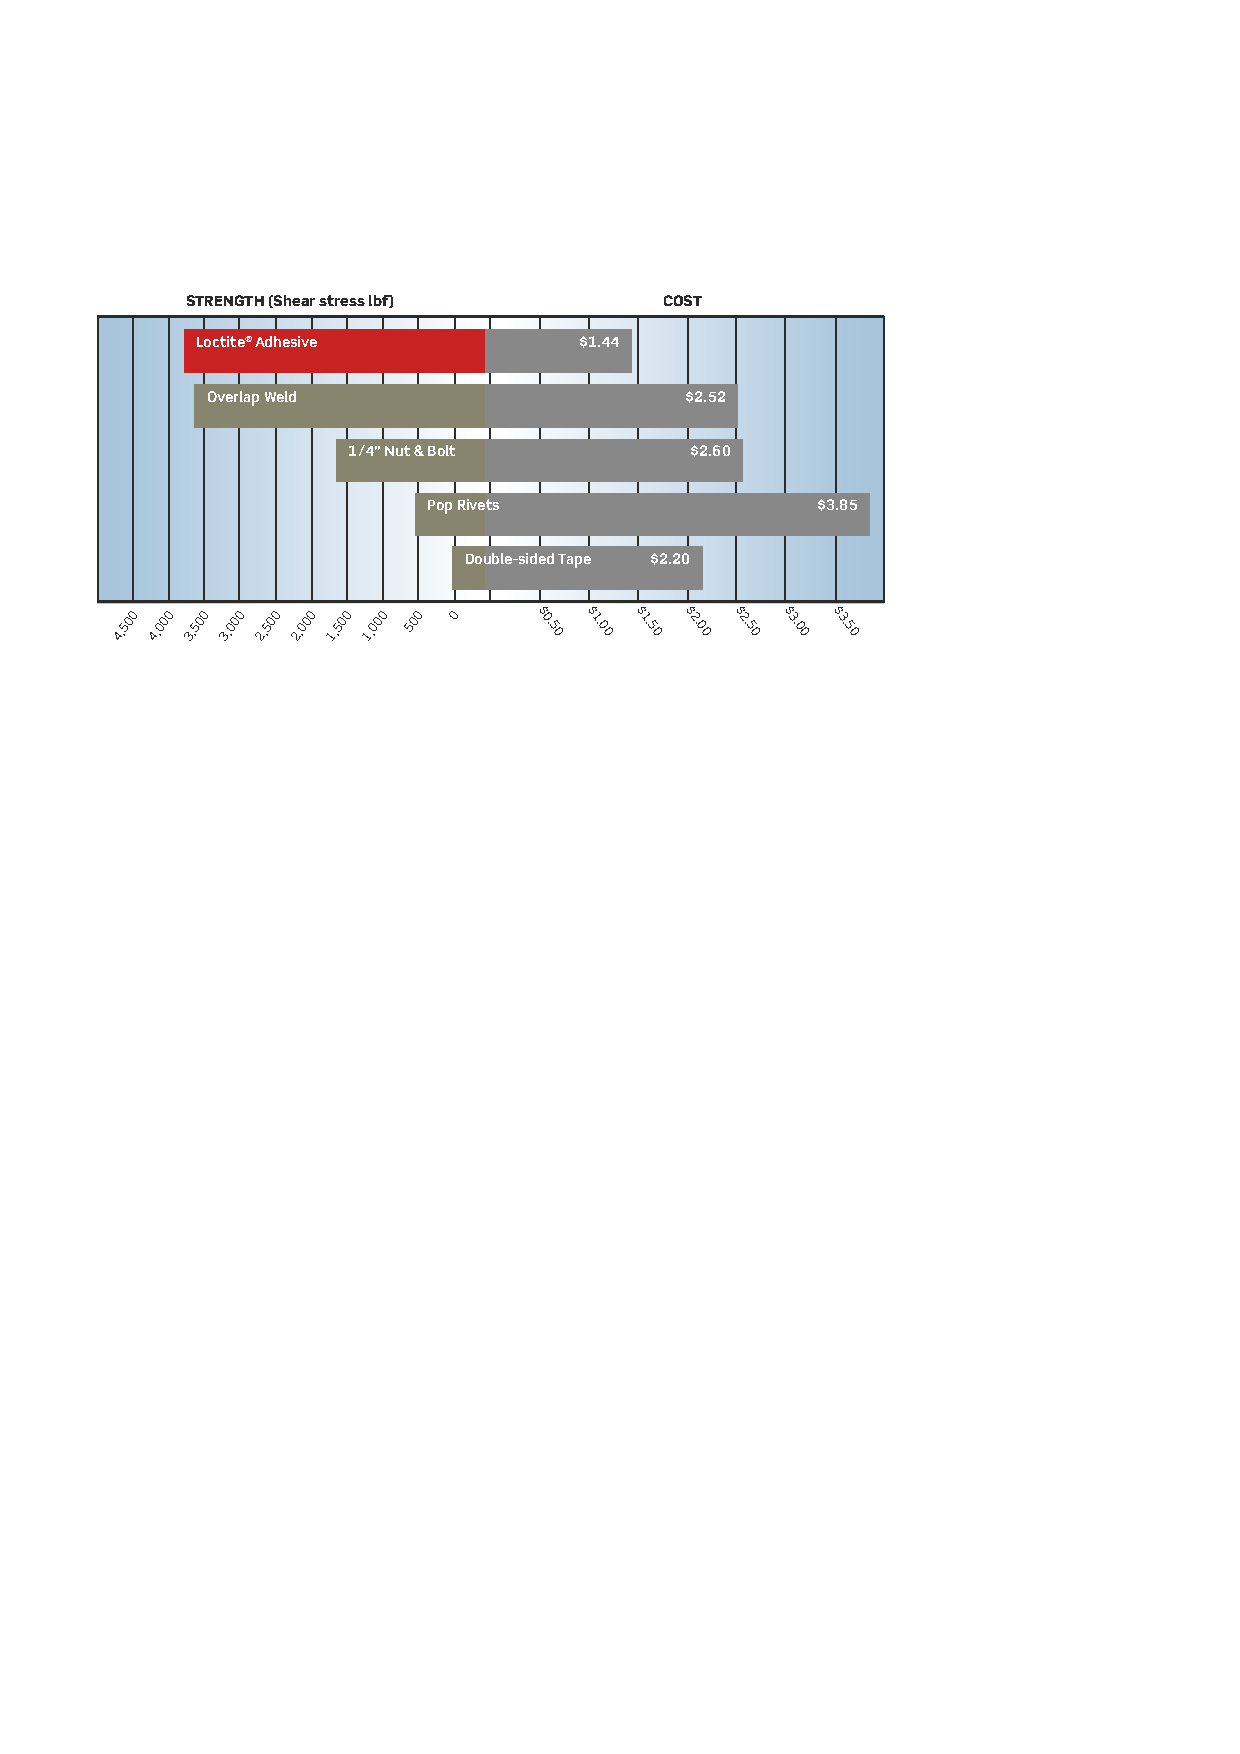
\includegraphics[width=0.7\linewidth]{./figures/IMG_CUTRES/comparison}
	\caption[Qualitative strength and cost comparison of different joining solutions.]{Qualitative strength and cost comparison of different joining solutions. Taken from \cite{superyacht}.}
	\label{fig:comparison}
\end{figure}

As \cref{fig:comparison} illustrates, adhesives are very competitive both in bonding strength and in economical manufacturing costs \cite{superyacht}. Although other solutions, like welding, may compete in strength, adhesives are much more inexpensive than other solutions. It should be recalled that this figure only aims to give a qualitative idea of this comparison for a particular manufacturer's point of view, and should not be taken as a fact.

In order to check adhesive's suitability for their use in crashworthy elements, this study develops numerical models of adhesively bonded crash boxes subjected to impact load  using the FEM. Information and data present in the literature are used to create and validate these models in order to ensure the accuracy of the results.

The present study aims to:

\begin{itemize}
	\item Determining an efficient adhesive modellization for its use in numerical models of adhesive joints. This modellization would also serve for studying hybrid bonding which implies the use of adhesives with other bonding solutions at the same time, such as welding or riveting.

	\item Checking the suitability of adhesives for their use in crash boxes or as a manner of improving other union types performance in that same devices.

	\item Generating a parametric model that would serve for sensitivity analysis and  optimization of the tube geometry by using the scripting capabilities of the finite element package employed.
\end{itemize}

In this introductory chapter, the most remarkable adhesive properties of interest are commented, along with experimental and numerical analysis that have been performed in the literature, with a later focus on their use in the field of crash boxes.

The present document is structured in three more chapters beyond this point, explaining the realized model, discussing the obtained results and drawing some conclusions, respectively. Two appendices are added at the end including some other aspects, such as the Python code developed for this study or the manufacturer's catalog information regarding to the selected adhesive.

\section{Finite element model}
\cite{brebbia84}
\todo{Poner bien las referencias (citet pero que funcione)}
\section{Optimization strategy}
\section{Conclusions}
\todo{Quitar el usepackage todonotes}
\section{Acknowledgments}



\bibliography{./references/references}

\end{document}
